\documentclass[10pt]{beamer}

\usetheme{metropolis}
\usepackage{appendixnumberbeamer}

\usepackage{booktabs}
\usepackage[scale=2]{ccicons}

\usepackage{pgfplots}
\usepgfplotslibrary{dateplot}

\usepackage{xspace}

\usepackage{tikz}
    \usetikzlibrary{positioning}

%\usepackage{listings}
\usepackage{minted}

\usepackage{bm}%................................. Bold math symbols (after fonts)

\setbeamercolor{normal text}{bg=white}





\title{EML4930/EML6934: Lecture 07}
\subtitle{Statistical distributions and functions with scipy.stats }
\date{October 12, 2017}
%\author{CJ}
\author{Charles Jekel}
%\titlegraphic{\includegraphics{images/avatarCropped.png}\vspace{58cm}}
%\institute{1. University of Florida\\ 2. Stellenbosch University, South Africa}

% \titlegraphic{\hfill\includegraphics[height=1.5cm]{logo.pdf}}

\begin{document}

\maketitle

\begin{frame}{Supplementary textbook for statistics in Python}
Freely available.

Think Stats by Allen B. Downey.
Exploratory Data Analysis in Python.

\url{http://greenteapress.com/wp/think-stats-2e/}
\end{frame}

\begin{frame}{Statistics with scipy.stats}

Today we're going to discuss many features of scipy.stats

The full documentation is available:
\url{https://docs.scipy.org/doc/scipy/reference/stats.html}

Part of this lecture will cover the tutorial here:
\url{https://docs.scipy.org/doc/scipy/reference/tutorial/stats.html}
\end{frame}

\begin{frame}{What will we cover today}
\begin{itemize}
\item Random variable distributions
\item Continuous and discrete distributions
\item PDF, CDF, SF, and other associated functions of distributions
\item Maximum likelihood estimation to fit distributions to data
\item Hypothesis test: are two samples from the same distribution?
\item Hypothesis test: are these samples from this distribution?
\end{itemize}
\end{frame}

\begin{frame}[fragile]{Reminder of viewing documentation}
In Python the documentation is included with the library.
\begin{minted}
{python}
from scipy import stats
# documentation of the namespace one screen at a time
stats?
# print the entire documentation
print(stats.__doc__)
# Don't forget the help function
help(stats)
# for a particular function
stats.norm?
# or
print(stats.norm.__doc__)
# __doc__ is a built in attribute created from the 
# comments following your function definition!
# view all of the contents in scipy.stats
dir(stats)
\end{minted}
\end{frame}

\begin{frame}{scipy.stats at a glance}
\begin{itemize}
\item 95 continuous distributions
\item 13 discrete distributions
\item 9 multivariate distributions
\item A number of other statistical functions and methods
\end{itemize}
\end{frame}

\begin{frame}{Common methods for continuous random variable distributions}
\begin{table}
\begin{tabular}{ll}
\textbf{Method} & \textbf{Description}  \\
\hline
    rvs & Random Variates \\
    pdf & Probability Density Function \\
    cdf & Cumulative Distribution Function \\
    sf & Survival Function (1-CDF) \\
    ppf & Percent Point Function (Inverse of CDF) \\
    isf & Inverse Survival Function (Inverse of SF)  \\
    stats & Return mean, variance, (Fisher’s) skew, or (Fisher’s) kurtosis \\
    moment & non-central moments of the distribution \\
\end{tabular}
\end{table}
\end{frame}

\begin{frame}[fragile]{scipy.stats namespace}
\begin{minted}
{python}
from scipy import stats

# the namespace follows:
# scipy.stats.distribution.method()

# demonstrating how to access methods of the 
# Maxwell continuous distribution
stats.maxwell.rvs()
stats.maxwell.pdf(1)
stats.maxwell.cdf(1)
stats.maxwell.sf(1)
stats.maxwell.ppf(0.5)

\end{minted}
\end{frame}

\begin{frame}[fragile]{It's safe to import the distributions themselves}
If you're only going to use a few functions and distributions, it may make sense to import them directly.
\begin{minted}
{python}
from scipy.stats import norm
from scipy.stats import binom
from scipy.stats import poisson

# now we can call the distributions directly
norm.pdf(0.9)

binom.cdf(8,n=100,p=0.1)

poisson.rvs(1)
\end{minted}
\end{frame}

\begin{frame}{Basic methods take vectorized input}
Basic methods such as pdf, and cdf are vectorized with np.vectorize.


pdf(0.5) will calculate the pdf at 0.5


cdf(0.5) will calculate the cdf at 0.5


However often we want to calculate the pdf and cdf at more than one value. For these cases we pass a numpy array of values into the functions.


pdf(x) will return an array of the same shape x of the pdf value of each item in x


\end{frame}

\begin{frame}[fragile]{Let's take a look at the normal distribution}
\mint{python}|scipy.stats.norm|
 scipy.stats.\_continuous\_distns.norm\_gen object
 A normal continuous random variable.

The location (loc) keyword specifies the mean. The scale (scale) keyword specifies the standard deviation.

\begin{minted}
{python}
import matplotlib.pyplot as plt
x = np.linspace(-3,3,100)
# the default normal distribution has a mean of 0
# and standard deviation of 1
y = norm.pdf(x)
plt.figure()
plt.plot(x,y)
plt.show()
\end{minted}
\end{frame}

\begin{frame}[fragile]{We can specify the mean and standard deviation}
\begin{minted}
{python}
mu = 2.0
std = 2.0
x = np.linspace(-4.0,8.0,100)
y = norm.pdf(x, mu, std)
z = norm.cdf(x, mu, std)
w = norm.sf(x, mu, std)

# plot the pdf, cdf, and sf
plt.figure()
plt.plot(x,y)
plt.plot(x,z)
plt.plot(x,w)
plt.show()
\end{minted}
\end{frame}

\begin{frame}{Digression: Meaning of PDF, CDF, and SF}
These are for continuous random variable $x$.
\smallskip
\smallskip

PDF - probability density function

PDF tells you the probability of a particular random variate occurring.
P($x = 0.5$) = PDF(0.5)

\smallskip
\smallskip

CDF - cumulative distribution function

CDF tells you the probability of a particular random variate being less than or equal to a value.

P($-\infty < t \leq m $) = CDF($m$) = $\int_{-\infty}^{m} PDF(t) dt$

P($ -\infty < x\leq 0.5$) = CDF(0.5)
\smallskip
\smallskip


SF - survival function

SF tells you the probability of a particular random variate being greater than a value.

P($x > 0.5$) = SF(0.5) = 1 - CDF(0.5)
\smallskip
\smallskip
\end{frame}

\begin{frame}[fragile]{Back to the normal distribution}
It's tedious to always specify the $mu, \sigma$ for each function. So what we do is create a \textit{Frozen} instance of the object. You won't be able to change the $mu, \sigma$ of the \textit{Frozen} instance.

\begin{minted}
{python}
mu1 = 2.0; std1 = 2.0
mu2 = 3.0; std2 = 1.0

# create a frozen normal distribution object
# from mu1, std1
my_norm1 = norm(mu1,std1)

# create a second frozen normal distribution object
my_norm2 = norm(mu2,std2)
\end{minted}
\end{frame}

\begin{frame}[fragile]{Working with a \textit{Frozen} instance}
\begin{minted}
{python}
# you'll see this will have all of the functions of norm
print(dir(my_norm1))

# let's plot the pdf of my_norm1 and my_norm2
x = np.linspace(-4.0,8.0,100)
plt.figure()
plt.plot(x, my_norm1.pdf(x))
plt.plot(x, my_norm2.pdf(x))
plt.show()
\end{minted}
\end{frame}

\begin{frame}[fragile]{Working with a \textit{Frozen} instance: generating random variables}
We can use the \textit{rvs} method to generate samples of random variables. The random generation relies on numpy's pseudorandom number generator. This means we can seed the random number generator to ensure the result is reproducible. 

\begin{minted}
{python}
# seed the random number generator
np.random.seed(1012301)

# generate 100 samples from my_norm1
rv1 = my_norm1.rvs(100)
# generate 10000 samples from my_norm2
rv2 = my_norm2.rvs(10000)

\end{minted}
\end{frame}

\begin{frame}[fragile]{Compare the histogram of the generated samples to the pdf}
\begin{minted}
{python}
# plot the histogram of the random samples and compare 
# to the pdf values

plt.figure()
plt.hist(rv1, normed=True)
plt.hist(rv2, bins=30, normed=True)
plt.plot(x, my_norm1.pdf(x))
plt.plot(x, my_norm2.pdf(x))
plt.show()
\end{minted}
\end{frame}

\begin{frame}[fragile]{Compare cumulative distribution of samples to the cdf}
\begin{minted}
{python}
# plot the cumulative histogram of the samples 
# and compare with the true cdf 

plt.figure()
plt.hist(rv1, cumulative=True, normed=True)
plt.hist(rv2, bins=30, cumulative=True, normed=True)
plt.plot(x, my_norm1.cdf(x))
plt.plot(x, my_norm2.cdf(x))
plt.show()
\end{minted}
\end{frame}

\begin{frame}[fragile]{What does the following code do?}
Does this code generate 10 samples from the normal distribution? 
\mint{python}|norm.rvs(10)|
... \textbf{Be careful!}
\end{frame}

\begin{frame}[fragile]{Be explicit by providing specifying the keywords}
Use the \textit{size} keyword to specify the number of samples to generate from a distribution.

The following code will produce the same random samples
\begin{minted}
{python}
np.random.seed(82)
aa = norm.rvs(10,3,1000)

np.random.seed(82)
bb = norm.rvs(loc=10, scale=3, size=1000)
# is aa exactly equal to bb?
print((aa == bb).all())

# if you specify the keywords, you can change the order
np.random.seed(82)
cc = norm.rvs(size=1000, loc=10, scale=3) 
# is cc exactly equal to bb?
print((cc == bb).all())
\end{minted}
\end{frame}

\begin{frame}[fragile]{Continuous distributions in general}
Use \textit{loc} and \textit{scale} to shift and scale distributions. However some distributions require additional shape parameters. To view the number of additional shape parameters use
\mint{python}|distrubituion_name.numargs|

Some examples:
\begin{minted}
{python}
in : print(stats.norm.numargs)
out: 0

in : print(stats.gamma.numargs)
out: 1

in : print(stats.beta.numargs)
out: 2
\end{minted}
\textbf{Note}: there is not a shape keyword.
\end{frame}

\begin{frame}[fragile]{How do you figure out how to specify the shape parameters?}
\mint{python}|stats.beta?|
\begin{figure}
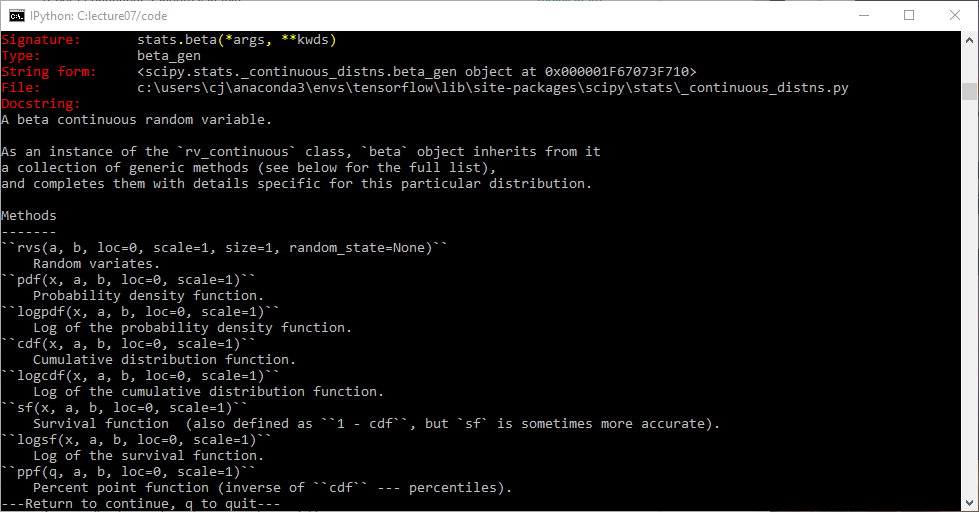
\includegraphics[width=1.0\textwidth]{figs/betaDist.png}
\end{figure}
The shape parameters for the beta random variate distribution are $a$ and $b$. In this case the order of the shape parameters matters!
\end{frame}

\begin{frame}{Methods for fitting distributions}
You most often use \textit{fit} to perform a maximum likelihood estimation of a distribution's parameters. Maximum likelihood estimations (MLE) can be very ill-posed, so it's recommended to provide \textit{fit} with a reasonable starting point.
\begin{table}
\begin{tabular}{ll}
\textbf{Method} & \textbf{Description}  \\
\hline
    fit & maximum likelihood estimation of parameters\\
    fit\_loc\_scale & estimation of loc and scale provided shape parameters\\
    nnlf & negative log likelihood function\\
    expect & Calculate the expectation of a function against the pdf or pmf\\
\end{tabular}
\end{table}
\textbf{Note}: these methods aren't available for every distribution
\end{frame}

\begin{frame}{From the tutorial: Performance issues and cautionary remarks}
\begin{itemize}
\item the performance of each distribution is different
\item some methods within distributions are explicitly calculated (by evaluating an analytic expression)
\item others are calculated with more costly methods if there is no analytically form (ie using generic algorithms)
\item MLE isn't a good choice for some distributions
\end{itemize}
\end{frame}

\begin{frame}[fragile]{You can build your own distributions using Subclassing}
Making a continuous distribution is simple and many values will be computed automatically.
\begin{minted}
{python}
from scipy import stats
class deterministic_gen(stats.rv_continuous):
    def _cdf(self, x):
        return np.where(x < 0, 0., 1.)
    def _stats(self):
        return 0., 0., 0., 0.
\end{minted}
\end{frame}

\begin{frame}{Whats different with discrete distributions?}
\begin{itemize}
\item Discrete distributions don't have a pdf, however they do have a pmf (probability mass function)
\item No estimation methods such as \textit{fit}
\item \textit{scale} is not valid, but \textit{loc} still is
\item cdf is a step function, thus inverse cdf (ppf) works a little bit differently
\begin{equation}
\text{ppf}(q) = \min (x: \text{cdf} (x) \geq q, x \text{integer}) 
\end{equation}
\end{itemize}
\end{frame}

\begin{frame}[fragile]{Enter the binomial distribution}
\begin{minted}
{python}
from scipy.stats import binom
# binom requires two arguments, n and p
n = 100   # number of trials
p = 1./6. # probability that you win

my_binom = binom(n,p)

n_wins = np.arange(0,40,1)
plt.figure()
plt.plot(n_wins,my_binom.pmf(n_wins), 'o')
plt.show()

# what is the proability that you'll win at least 16 times?
print(my_binom.sf(15))

# what is the probability that you won't win more than 25 times? 
print(my_binom.cdf(24))
\end{minted}
\end{frame}

\begin{frame}[fragile]{Example: fitting a distribution 1 of 3}
\begin{minted}
{python}
# let's generate random samples from a normal distribution
# and fit a beta distribution to the samples

np.random.seed(467)
rv = norm.rvs(loc=4.0,scale=1.0,size=10000)

# estimate the mean and variance
est_loc = np.mean(rv)
est_scale = np.std(rv)

# perform the MLE to determine the beta parameters
beta_param = stats.beta.fit(rv, loc=est_loc, scale=est_scale)

# create the beta model
beta_fit = stats.beta(*beta_param)
# equiv to stats.beta(beta_param[0], beta_param[1], ...
\end{minted}
\end{frame}

\begin{frame}[fragile]{Example: fitting a distribution 2 of 3}
\begin{minted}
{python}
# let's compare the pdf from the fitted beta distribution
# to the histogram of the samples

x = np.linspace(1.0, 7.0, 100)

plt.figure()
plt.hist(rv, bins=30, normed=True)
plt.plot(x, beta_fit.pdf(x))
plt.show()

# and the cdf to the cumulative histogram
plt.figure()
plt.hist(rv, bins=30, cumulative=True, normed=True)
plt.plot(x, beta_fit.cdf(x))
plt.show()
\end{minted}
\end{frame}

\begin{frame}[fragile]{Example: fitting a distribution 3 of 3}
\begin{minted}
{python}
# we can use the Kolmogorov-Smirnov test to perform a 
# hypothesis test to see if our samples do come from beta

# Hypothesis: the rv does indeed come from beta distribution
# for 99% confidence reject if pvalue is less than 0.01

test_res = stats.kstest(rv, 'beta', beta_param)
print('KS-statistic D = %6.3f pvalue = %6.4f' % test_res )

# is this better than a ufitted normal estimate?
test_norm = stats.kstest(rv, 'norm', (np.mean(rv), np.std(rv)))
print('KS-statistic D = %6.3f pvalue = %6.4f' % test_norm )
\end{minted}
\textbf{Note}: Dont' use pvalues to deice if anything is quantitative better than anything else! The pvalue is just an accept or reject of the hypothesis. 
\end{frame}

\begin{frame}[fragile]{Kolmogorov-Smirnov test for two sample}
This is a hypothesis test for to determine whether two sets of samples originate from the same distribution. 

Hypotheses: The samples come from the same distribution.
Reject if he hypothesis when the pvalue is small.
\begin{minted}
{python}
np.random.seed(1212)
rvs1 = stats.norm.rvs(loc=5, scale=10, size=500)
rvs2 = stats.norm.rvs(loc=5, scale=10, size=100)
rvs3 = stats.norm.rvs(loc=4, scale=14, size=200)

# test wheter 1 and 2 come from the same distribution
# for 95% confidece we reject if the pvalue is less than 0.05

test_12 = stats.ks_2samp(rvs1, rvs2)
test_13 = stats.ks_2samp(rvs1, rvs3)
test_23 = stats.ks_2samp(rvs2, rvs3)

\end{minted}
\end{frame}

\begin{frame}{So what did we cover today}
\begin{itemize}
\item Introduction to statistics with scipy.stats
\item How the object oriented frozen distributions work
\item Random variable distributions
\item Continuous and discrete distributions
\item PDF, CDF, SF, and other associated functions of distributions
\item Maximum likelihood estimation to fit distributions to data
\item Hypothesis test: are two samples from the same distribution?
\item Hypothesis test: are these samples from this distribution?
\end{itemize}
\end{frame}

\begin{frame}{So whats still out there?}
\begin{itemize}
\item There is a lot more that we can't cover in one day...
\item We can make an entire class on statistics in Python
\item We didn't cover multivariate distributions...
\item There are numerous other functions in scipy.stats
\item There are plotting tools in scipy.stats (probability plots, box plots, etc.)
\end{itemize}
\end{frame}



%\begin{frame}{Reminder Quiz at the end of this class}
%
%\end{frame}
%
%\begin{frame}{Issues with HW?}
%
%\end{frame}
%
%\begin{frame}{What am I going to cover this lecture}
%\begin{itemize}
%\item review arrays
%\item difference between array dimensions
%\item array shaping
%\item saving and loading numpy arrays
%\item matplotlib 
%\end{itemize}
%\end{frame}
%
%\begin{frame}[fragile]{Let's consider these two arrays}
%\begin{minted}
%{python}
%import numpy as np
%a = np.array([6, 9, 2, 3, 6])
%b = np.array([[6], [9], [2], [3], [6]])
%
%# what are the dimensions
%print(a.ndim)
%print(b.ndim)
%
%# what are the shapes
%print(a.shape)
%print(b.shape)
%
%# let's print the transpose of a
%print(a)
%print(a.T)
%
%\end{minted}
%\end{frame}
%
%\begin{frame}[fragile]{Let's consider these two arrays}
%\begin{minted}
%{python}
%# let's print the transpose of b
%c = b.T
%print(b)
%print(c)
%
%# what has change?
%print(b.shape)
%print(c.shape)
%
%# what is the difference between the following?
%print(a*a)
%print(np.dot(a,a))
%\end{minted}
%\end{frame}
%
%\begin{frame}[fragile]{Saving NumPy arrays}
%\mint{python}|np.save(file, arr)|
%Save an array to a binary file in NumPy .npy format.
%\mint{python}|np.save('a_vect',a)|
%This creates a\_vect.npy file of the vector a.
%\end{frame}
%
%\begin{frame}[fragile]{Loading NumPy arrays}
%\mint{python}|np.load(file)|
%Load arrays or pickled objects from .npy, .npz or pickled files.
%\mint{python}|a_vect = np.load('a_vect.npy')|
%This loads the a\_vect.npy binary file into the a\_vect vector.
%\end{frame}
%
%\begin{frame}[fragile]{Saving NumPy arrays as plain text and loading the file}
%\mint{python}|np.savetxt(fname,X)|
%Save the array X to a text file fname.
%\mint{python}|a = numpy.loadtxt(fname)|
%Load data from a text file named fname and store this as array a.
%
%Each row in the text file must have the same number of values.
%\end{frame}
%
%\begin{frame}[fragile]{NumPy reshape}
%\begin{minted}
%{python}
%a = np.arange(6)
%b = a.reshape((3,2))
%c = a.reshape((2,3))
%d = a.reshape((6,1))
%print(b)
%print(c)
%print(d)
%
%out:
%[[0 1]
% [2 3]
% [4 5]]
%[[0 1 2]
% [3 4 5]]
%[[0 1 2 3 4 5]]
%\end{minted}
%\end{frame}
%
%\begin{frame}[fragile]{NumPy array concatenation - or joining}
%\begin{minted}
%{python}
%x = np.array([4, 5, 0, 3, 7])
%y = np.array([3, 4, 9, 7, 5])
%z = np.concatenate([x,y])
%print(z)
%
%# you can you use np.vstack to vertically stack arrays
%w = np.vstack([x,y])
%
%# you can use np.hstack to horizontally stack arrays
%v = np.hstack([w,w])
%\end{minted}
%\end{frame}
%
%\begin{frame}[fragile]{flatten any ndarray into one dimension}
%\begin{minted}
%{python}
%k = np.random.random((5,3,2,6,8))
%print(k.ndim)
%k_flat = k.flatten()
%print(k_flat.ndim)
%print(k_flat.size)
%
%out:
%5
%1
%1440
%\end{minted}
%\end{frame}
%
%\begin{frame}{matplotlib}
%Matplotlib tries to make easy things easy and hard things possible. You can generate plots, histograms, power spectra, bar charts, errorcharts, scatterplots, etc., with just a few lines of code. For a sampling, see the screenshots, thumbnail gallery, and examples directory
%
%For simple plotting the pyplot module provides a MATLAB-like interface, particularly when combined with IPython. For the power user, you have full control of line styles, font properties, axes properties, etc, via an object oriented interface or via a set of functions familiar to MATLAB users.
%
%\url{https://matplotlib.org/}
%\end{frame}
%
%\begin{frame}{For reference}
%Dr. Jake VanderPlas’s Python Data Science Handbook: Essential Tools for Working with Data.
%
%Chapter 4: Visualization with Matplotlib
%
%\url{http://nbviewer.jupyter.org/github/jakevdp/PythonDataScienceHandbook/blob/master/notebooks/Index.ipynb}
%\end{frame}
%
%\begin{frame}[fragile]{matplotlib pyplot - MATLAB like plotting framework}
%\begin{minted}
%{python}
%import numpy as np
%import matplotlib.pyplot as plt
%
%x = np.linspace(0.0, 2.0*np.pi, 25)
%
%# you can specify a figure number or string name
%# but by default plt.figure() will create a number ordered 
%# figure name Ex: plt.figure('my figure') or plt.figure(1)
%plt.figure() 
%# create a line plot by default
%plt.plot(x,np.cos(x))
%# show the plot
%plt.show()
%\end{minted}
%\end{frame}
%
%\begin{frame}{matplotlib linestyles}
%\begin{table}
%\begin{tabular}{ll}
%\textbf{Linestyle} & \textbf{Description}  \\
%\hline
%'-' or 'solid' 	 &  solid line\\
%'--' or 'dashed' &	dashed line\\
%'-.' or 'dashdot'& 	dash-dotted line\\
%':' or 'dotted'  &	dotted line\\
%'None'           &	draw nothing\\
%' '              &	draw nothing\\
%'' 	             &  draw nothing\\
%\end{tabular}
%\end{table}
%\end{frame}
%
%\begin{frame}[fragile]{Plotting cosine with a dashed line}
%\begin{minted}
%{python}
%import numpy as np
%import matplotlib.pyplot as plt
%
%x = np.linspace(0.0, 2.0*np.pi, 25)
%
%plt.figure() 
%
%# all you need to do is pass the linestyle as an attribute
%plt.plot(x,np.cos(x), '--')
%plt.show()
%\end{minted}
%\end{frame}
%
%\begin{frame}{Scatter plot markers}
%and more at - \url{https://matplotlib.org/api/markers_api.html} 
%\begin{table}
%\begin{tabular}{ll}
%\textbf{Marker} & \textbf{Description}  \\
%\hline
%"." &	point\\
%"," &	pixel\\
%"o" &	circle\\
%"v" &	triangle\_down\\
%"$<$" &	triangle\_left\\
%"$>$" &	triangle\_right\\
%"1" &	tri\_down\\
%"2" &	tri\_up\\
%"3" &	tri\_left\\
%"4" &	tri\_right\\
%"8" &	octagon\\
%"s" &	square\\
%"p" &	pentagon\\
%"P" &	plus (filled)\\
%\end{tabular}
%\end{table}
%\end{frame}
%
%\begin{frame}[fragile]{Scatter plot cosine}
%\begin{minted}
%{python}
%import numpy as np
%import matplotlib.pyplot as plt
%
%x = np.linspace(0.0, 2.0*np.pi, 25)
%
%plt.figure() 
%
%# all you need to do is pass the marker into plot
%plt.plot(x,np.cos(x), 'o')
%plt.show()
%\end{minted}
%\end{frame}
%
%\begin{frame}[fragile]{You can easily combine markers and linestyles}
%\begin{minted}
%{python}
%import numpy as np
%import matplotlib.pyplot as plt
%
%x = np.linspace(0.0, 2.0*np.pi, 25)
%
%plt.figure() 
%
%# this will plot a -- linestyle with circles at the data points
%plt.plot(x,np.cos(x), '--o')
%plt.show()
%\end{minted}
%\end{frame}
%
%\begin{frame}{basic built-in colors in matplotlib}
%and more at - \url{https://matplotlib.org/api/colors_api.html} 
%\begin{table}
%\begin{tabular}{ll}
%\textbf{Code} & \textbf{Color}  \\
%\hline
%b & blue\\
%g & green\\
%r & red\\
%c & cyan\\
%m & magenta\\
%y & yellow\\
%k & black\\
%w & white\\
%\end{tabular}
%\end{table}
%\end{frame}
%
%\begin{frame}[fragile]{You can specify the built in color into plot}
%\begin{minted}
%{python}
%import numpy as np
%import matplotlib.pyplot as plt
%
%x = np.linspace(0.0, 2.0*np.pi, 25)
%
%plt.figure() 
%
%# forcing the line and dot color to be blue
%plt.plot(x,np.cos(x), 'b--o')
%plt.show()
%\end{minted}
%\end{frame}
%
%\begin{frame}[fragile]{Alternatively use color=''}
%\begin{minted}
%{python}
%# specify color by name 
%plt.plot(x, np.cos(x), color='blue')
%
%# short color code (rgbcmyk)
%plt.plot(x, np.cos(x), color='g') 
%
%# Grayscale between 0 and 1                   
%plt.plot(x, np.cos(x), color='0.75')        
%
%# Hex code (RRGGBB from 00 to FF) 
%plt.plot(x, np.cos(x), color='#FFDD44')     
%
%# RGB tuple, values 0 and 1 
%plt.plot(x, np.cos(x), color=(1.0,0.2,0.3)) 
%
%# all HTML color names supported
%plt.plot(x, np.cos(x), color='chartreuse') 
%\end{minted}
%\end{frame}
%
%\begin{frame}[fragile]{Adjusting the plot with axes limit}
%\begin{minted}
%{python}
%import numpy as np
%import matplotlib.pyplot as plt
%
%x = np.linspace(0.0, 2.0*np.pi, 25)
%
%plt.figure() 
%plt.plot(x,np.cos(x), 'b--o')
%
%# set the x axis limit
%plt.xlim(-1,7)
%
%# set the y axis limit
%plt.ylim(-2,2)
%
%plt.show()
%\end{minted}
%\end{frame}
%
%\begin{frame}[fragile]{Adding a grid}
%\url{https://matplotlib.org/api/pyplot_api.html?highlight=matplotlib%20pyplot%20grid#matplotlib.pyplot.grid}
%
%grid(b=None, which='major', axis='both', **kwargs)
%
%    kwargs are used to set the grid line properties, e.g.,:
%    \mint{python}|ax.grid(color='r', linestyle='-', linewidth=2)|
%\begin{minted}
%{python}
%import numpy as np
%import matplotlib.pyplot as plt
%x = np.linspace(0.0, 2.0*np.pi, 25)
%plt.figure() 
%plt.plot(x,np.cos(x), 'b--o')
%# create a grid
%plt.grid(True)
%plt.show()
%\end{minted}
%\end{frame}
%
%\begin{frame}[fragile]{Labels and legend}
%\begin{minted}
%{python}
%import numpy as np
%import matplotlib.pyplot as plt
%x = np.linspace(0.0, 2.0*np.pi, 25)
%plt.figure() 
%
%# add label='my_label'
%plt.plot(x,np.cos(x), '--o', label='cos')
%plt.plot(x,np.sin(x), '-.s', label='sin')
%plt.grid(True)
%
%# add legend
%plt.legend()
%# legend automatically chooses the location
%# but you can specify the simple quadrant based location as
%# plt.legend(loc=1) puts the legend in the first quadrant
%
%plt.show()
%\end{minted}
%\end{frame}
%
%\begin{frame}[fragile]{matplotlib title and axis label}
%\begin{minted}
%{python}
%import numpy as np
%import matplotlib.pyplot as plt
%x = np.linspace(0.0, 2.0*np.pi, 25)
%plt.figure() 
%plt.plot(x,np.cos(x), '--o', label='cos')
%plt.plot(x,np.sin(x), '-.s', label='sin')
%plt.grid(True)
%plt.legend()
%# adding a title
%plt.title('Cos and sin')
%
%# x and y axis labels
%plt.xlabel('x axis')
%plt.ylabel('y axis')
%
%plt.show()
%\end{minted}
%\end{frame}
%
%\begin{frame}[fragile]{matplotlib pyplot savefig}
%\url{https://matplotlib.org/api/pyplot_api.html?highlight=matplotlib%20pyplot%20savefig#matplotlib.pyplot.savefig}
%
%\begin{minted}
%{python}
%plt.savefig(fname, dpi=None, facecolor='w', edgecolor='w',
%        orientation='portrait', papertype=None, format=None,
%        transparent=False, bbox_inches=None, pad_inches=0.1,
%        frameon=None)
%\end{minted}
%
%How I normally create publication quality pictures:
%\begin{minted}
%{python}
%plt.savefig('my_fig.pdf', dpi=600, format='pdf',
%            bbox_inches='tight')
%\end{minted}
% Most backends support png, pdf, ps, eps and svg.
%\end{frame}
%
%\begin{frame}[fragile]{saving my cosine and sin plot}
%Depending on your active Python interpreter, you'll have issues with plt.show()
%\begin{minted}
%{python}
%import numpy as np
%import matplotlib.pyplot as plt
%x = np.linspace(0.0, 2.0*np.pi, 25)
%plt.figure() 
%plt.plot(x,np.cos(x), '--o', label='cos')
%plt.plot(x,np.sin(x), '-.s', label='sin')
%plt.grid(True)
%plt.legend()
%plt.xlabel('x axis')
%plt.ylabel('y axis')
%
%plt.savefig('my_fig.pdf', dpi=600, format='pdf',
%             bbox_inches='tight')
%\end{minted}
%\end{frame}
%
%\begin{frame}{Created this plot}
%\begin{figure}
%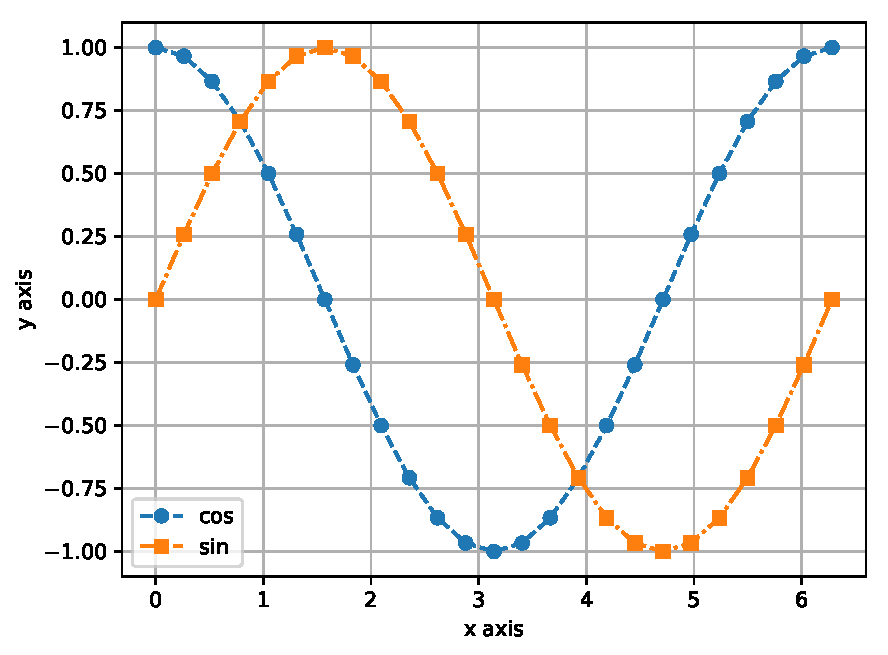
\includegraphics[width=0.9\textwidth]{fig/my_fig.pdf}
%\end{figure}
%\end{frame}


\end{document}
